%!TEX program = pdflatex
\documentclass[aspectratio=169,10pt]{beamer}

% Theme - Colorblind friendly
\usetheme{default}
\usecolortheme{dolphin}
\usefonttheme{structurebold}

% Packages
\usepackage{graphicx}
\usepackage{listings}
\usepackage{xcolor}
\usepackage{tikz}
\usepackage{booktabs}
% \usepackage{fontawesome5} % Commented out - may not be available
\usetikzlibrary{shapes,arrows,positioning}

% Okabe-Ito colorblind-friendly palette
\definecolor{OkabeOrange}{RGB}{230,159,0}
\definecolor{OkabeSkyBlue}{RGB}{86,180,233}
\definecolor{OkabeGreen}{RGB}{0,158,115}
\definecolor{OkabeYellow}{RGB}{240,228,66}
\definecolor{OkabeBlue}{RGB}{0,114,178}
\definecolor{OkabeVermillion}{RGB}{213,94,0}
\definecolor{OkabePurple}{RGB}{204,121,167}
\definecolor{OkabeGray}{RGB}{128,128,128}

% Additional colors for syntax highlighting
\definecolor{CodeBgGray}{RGB}{248,248,248}
\definecolor{CommentGray}{RGB}{96,96,96}
\definecolor{StringRed}{RGB}{213,94,0}  % Okabe Vermillion

% Code listing styles - Colorblind friendly with distinct themes
\lstdefinestyle{bashstyle}{
    language=bash,
    basicstyle=\ttfamily\small,
    keywordstyle=\color{OkabeBlue}\bfseries,      % Blue for keywords
    commentstyle=\color{CommentGray}\itshape,      % Gray for comments
    stringstyle=\color{OkabeOrange},               % Orange for strings
    backgroundcolor=\color{CodeBgGray},
    identifierstyle=\color{black},
    frame=single,
    framerule=0.5pt,
    rulecolor=\color{OkabeGray},
    breaklines=true,
    showstringspaces=false,
    xleftmargin=0.5cm,
    xrightmargin=0.5cm,
    numbers=none,
    numberstyle=\tiny\color{OkabeGray},
    tabsize=4,
    columns=flexible
}

\lstdefinestyle{pythonstyle}{
    language=Python,
    basicstyle=\ttfamily\small,
    keywordstyle=\color{OkabeVermillion}\bfseries, % Vermillion for keywords
    commentstyle=\color{CommentGray}\itshape,       % Gray for comments
    stringstyle=\color{OkabeGreen},                 % Green for strings
    backgroundcolor=\color{CodeBgGray},
    identifierstyle=\color{black},
    emphstyle=\color{OkabePurple}\bfseries,        % Purple for special
    frame=single,
    framerule=0.5pt,
    rulecolor=\color{OkabeGray},
    breaklines=true,
    showstringspaces=false,
    xleftmargin=0.5cm,
    xrightmargin=0.5cm,
    numbers=none,
    numberstyle=\tiny\color{OkabeGray},
    tabsize=4,
    columns=flexible,
    % Python-specific highlighting
    morekeywords={self,True,False,None,as,with},
    emph={def,class,import,from,return},
    emphstyle=\color{OkabePurple}\bfseries
}

% Title page
\title{MMML: A Complete Machine Learning Pipeline for Molecular Modeling}
\subtitle{Command-Line Tools for Production-Ready ML Potentials}
\author{MMML Development Team}
\institute{Molecular ML Framework}
\date{\today}

\begin{document}

% Title slide
\begin{frame}
\titlepage
\end{frame}

% Table of contents
\begin{frame}{Outline}
\tableofcontents
\end{frame}

% ============================================================================
\section{Introduction}
% ============================================================================

\begin{frame}{What is MMML?}
\begin{columns}
\column{0.5\textwidth}
\textbf{Modern Molecular ML Framework}
\begin{itemize}
    \item Production-ready CLI tools
    \item PhysNet + DCMNet architectures
    \item Efficient data handling
    \item Comprehensive validation
    \item Multi-state predictions
\end{itemize}

\column{0.5\textwidth}
\begin{center}
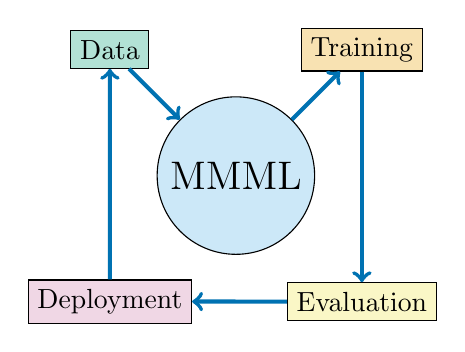
\begin{tikzpicture}[scale=0.8]
    % Central node - using Okabe-Ito colors
    \node[circle,draw,fill=OkabeSkyBlue!30,minimum size=2cm] (mmml) at (0,0) {\Large MMML};
    
    % Surrounding nodes with colorblind-friendly colors
    \node[rectangle,draw,fill=OkabeGreen!30] (data) at (-2,2) {Data};
    \node[rectangle,draw,fill=OkabeOrange!30] (train) at (2,2) {Training};
    \node[rectangle,draw,fill=OkabeYellow!30] (eval) at (2,-2) {Evaluation};
    \node[rectangle,draw,fill=OkabePurple!30] (deploy) at (-2,-2) {Deployment};
    
    % Arrows with thicker, more visible style
    \draw[->,line width=1.5pt,color=OkabeBlue] (data) -- (mmml);
    \draw[->,line width=1.5pt,color=OkabeBlue] (mmml) -- (train);
    \draw[->,line width=1.5pt,color=OkabeBlue] (train) -- (eval);
    \draw[->,line width=1.5pt,color=OkabeBlue] (eval) -- (deploy);
    \draw[->,line width=1.5pt,color=OkabeBlue] (deploy) -- (data);
\end{tikzpicture}
\end{center}
\end{columns}
\end{frame}

\begin{frame}{Key Features}
\begin{columns}
\column{0.33\textwidth}
\begin{block}{Data Processing}
\begin{itemize}
    \item Auto-padding removal
    \item Quality control
    \item Train/val/test splits
    \item Memory-mapped support
\end{itemize}
\end{block}

\column{0.33\textwidth}
\begin{block}{Model Training}
\begin{itemize}
    \item PhysNet (E/F/D)
    \item DCMNet (ESP)
    \item Multi-state (charge/spin)
    \item Auto-tuned hyperparams
\end{itemize}
\end{block}

\column{0.33\textwidth}
\begin{block}{Analysis Tools}
\begin{itemize}
    \item Model evaluation
    \item MD simulations
    \item Vibrational analysis
    \item ASE integration
\end{itemize}
\end{block}
\end{columns}
\end{frame}

% ============================================================================
\section{Data Preparation}
% ============================================================================

\begin{frame}[fragile]{Data Cleaning}
\textbf{Remove problematic structures from your dataset}

\begin{lstlisting}[style=bashstyle]
# Clean dataset with quality control
python -m mmml.cli.clean_data glycol.npz \
    -o glycol_cleaned.npz \
    --max-force 10.0 \
    --min-distance 0.4 \
    --max-energy -1e-3
\end{lstlisting}

\textbf{What it does:}
\begin{itemize}
    \item Removes zero/NaN/Inf energies
    \item Filters high forces (SCF failures)
    \item Checks for overlapping atoms
    \item Keeps only essential fields (E, F, R, Z, N, D)
\end{itemize}

\vspace{0.3cm}
\textbf{Result:} Clean, validated dataset ready for training
\end{frame}

\begin{frame}[fragile]{Data Exploration}
\textbf{Understand your dataset before training}

\begin{lstlisting}[style=bashstyle]
# Explore dataset statistics
python -m mmml.cli.explore_data glycol_cleaned.npz \
    --plot-distributions \
    --analyze-bonds \
    --output-dir analysis/
\end{lstlisting}

\textbf{Provides:}
\begin{columns}
\column{0.5\textwidth}
\begin{itemize}
    \item Energy distribution
    \item Force statistics
    \item Bond length analysis
    \item Molecular size distribution
\end{itemize}

\column{0.5\textwidth}
\begin{itemize}
    \item Element composition
    \item Distance matrices
    \item Quality metrics
    \item Summary statistics
\end{itemize}
\end{columns}

\vspace{0.3cm}
\textbf{Example output:} 5,782 structures, 10 atoms, C/H/O composition
\end{frame}

\begin{frame}[fragile]{Dataset Splitting}
\textbf{Create train/validation/test splits}

\begin{lstlisting}[style=bashstyle]
# Split dataset (80% train, 10% val, 10% test)
python -m mmml.cli.split_dataset glycol_cleaned.npz \
    -o splits/ \
    --train-size 0.8 \
    --valid-size 0.1 \
    --test-size 0.1 \
    --seed 42
\end{lstlisting}

\textbf{Features:}
\begin{itemize}
    \item Reproducible splits (seed-based)
    \item Filters out non-per-structure fields
    \item Saves split indices for reproducibility
    \item Stratified splitting available
\end{itemize}

\vspace{0.3cm}
\textbf{Output:} \texttt{data\_train.npz}, \texttt{data\_valid.npz}, \texttt{data\_test.npz}
\end{frame}

\begin{frame}[fragile]{Automatic Padding Removal}
\textbf{NEW: Training now auto-detects and removes padding!}

\begin{lstlisting}[style=bashstyle]
# Before: Dataset padded to 60 atoms (10 real + 50 padding)
# After: Automatically detected and removed during training

python -m mmml.cli.make_training \
    --data splits/data_train.npz \
    --ckpt_dir checkpoints/glycol
\end{lstlisting}

\textbf{Console output:}
\begin{lstlisting}[style=bashstyle,basicstyle=\ttfamily\tiny]
Auto-detecting number of atoms from dataset...
  ✅ Actual molecule size: 10 atoms (from max(N))
  ⚠️  Data is PADDED: 60 atoms (padding: 50)
  🔧 Auto-removing padding to train efficiently...
  ✅ Saved unpadded data to: data_train_unpadded.npz
\end{lstlisting}

\textbf{Result:} \textbf{6x faster training!} (10 vs 60 atoms)
\end{frame}

% ============================================================================
\section{Model Training}
% ============================================================================

\begin{frame}[fragile]{Basic Training}
\textbf{Train a PhysNet model for energies, forces, and dipoles}

\begin{lstlisting}[style=bashstyle]
# Simple training with auto-detection
python -m mmml.cli.make_training \
    --data splits/data_train.npz \
    --ckpt_dir checkpoints/glycol_run1 \
    --n_train 4000 \
    --n_valid 500 \
    --num_epochs 100 \
    --batch_size 16
\end{lstlisting}

\textbf{Auto-detected:}
\begin{itemize}
    \item Number of atoms (from dataset)
    \item Padding removal (if needed)
    \item Checkpoint path (made absolute)
\end{itemize}
\end{frame}

\begin{frame}[fragile]{Training Configuration}
\textbf{Customize your training with many options}

\begin{lstlisting}[style=bashstyle,basicstyle=\ttfamily\tiny]
python -m mmml.cli.make_training \
    --data splits/data_train.npz \
    --ckpt_dir checkpoints/glycol_production \
    --n_train 4000 --n_valid 500 \
    --num_epochs 100 --batch_size 16 \
    --learning_rate 0.001 --features 128 \
    --num_iterations 3 --cutoff 10.0 \
    --energy_weight 1.0 --forces_weight 1.0 \
    --dipole_weight 1.0
\end{lstlisting}

\begin{columns}
\column{0.5\textwidth}
\textbf{Model architecture:}
\begin{itemize}
    \item \texttt{--features}: Hidden size
    \item \texttt{--num\_iterations}: MP steps
    \item \texttt{--cutoff}: Interaction range
    \item \texttt{--num\_basis\_functions}: RBF
\end{itemize}

\column{0.5\textwidth}
\textbf{Loss weights:}
\begin{itemize}
    \item \texttt{--energy\_weight}
    \item \texttt{--forces\_weight}
    \item \texttt{--dipole\_weight}
    \item \texttt{--charges\_weight}
\end{itemize}
\end{columns}
\end{frame}

\begin{frame}[fragile]{Joint PhysNet+DCMNet Training}
\textbf{Advanced: Train for ESP prediction}

\begin{lstlisting}[style=bashstyle,basicstyle=\ttfamily\tiny]
# Train joint model for electrostatic potential
python -m mmml.cli.train_joint \
    --train-efd train_efd.npz \
    --train-esp train_esp.npz \
    --valid-efd valid_efd.npz \
    --valid-esp valid_esp.npz \
    --epochs 100 --batch-size 4 \
    --optimizer adamw --use-recommended-hparams
\end{lstlisting}

\textbf{Architecture:}
\begin{center}
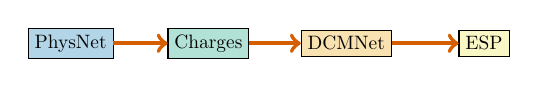
\begin{tikzpicture}[node distance=1.5cm,scale=0.7,transform shape]
    \node[rectangle,draw,fill=OkabeBlue!30] (physnet) {PhysNet};
    \node[rectangle,draw,fill=OkabeGreen!30,right of=physnet,xshift=1cm] (charges) {Charges};
    \node[rectangle,draw,fill=OkabeOrange!30,right of=charges,xshift=1cm] (dcmnet) {DCMNet};
    \node[rectangle,draw,fill=OkabeYellow!30,right of=dcmnet,xshift=1cm] (esp) {ESP};
    
    \draw[->,line width=1.5pt,color=OkabeVermillion] (physnet) -- (charges);
    \draw[->,line width=1.5pt,color=OkabeVermillion] (charges) -- (dcmnet);
    \draw[->,line width=1.5pt,color=OkabeVermillion] (dcmnet) -- (esp);
\end{tikzpicture}
\end{center}

\textbf{Features:}
\begin{itemize}
    \item Multiple optimizers (Adam, AdamW, RMSprop, Muon)
    \item Auto-tuned hyperparameters
    \item Comprehensive ESP validation plots
\end{itemize}
\end{frame}

\begin{frame}[fragile]{Memory-Mapped Training}
\textbf{Train on large datasets (\textgreater100k structures)}

\begin{lstlisting}[style=bashstyle]
# Train on memory-mapped data (no RAM limits)
python -m mmml.cli.train_memmap \
    --data_path openqdc_packed_memmap \
    --batch_size 32 \
    --num_epochs 100 \
    --num_atoms 60 \
    --bucket_size 8192
\end{lstlisting}

\textbf{Benefits:}
\begin{itemize}
    \item No RAM limits (memory-mapped)
    \item Bucketed batching (minimizes padding)
    \item HPC-friendly (efficient I/O)
    \item Scales to millions of structures
\end{itemize}

\textbf{Compatible with:} OpenQDC, custom packed formats
\end{frame}

\begin{frame}[fragile]{Multi-State Training}
\textbf{Train models for different charge and spin states}

\begin{lstlisting}[style=bashstyle]
# Train charge/spin conditioned model
python -m mmml.cli.train_charge_spin \
    --data_path openqdc_packed_memmap \
    --batch_size 32 \
    --charge_min -2 --charge_max 2 \
    --spin_min 1 --spin_max 5
\end{lstlisting}

\textbf{Applications:}
\begin{itemize}
    \item Ionic species (charge states)
    \item Excited states (spin states)
    \item Redox reactions
    \item Photochemistry
\end{itemize}

\textbf{Method:} Learned embeddings for charge and spin
\end{frame}

% ============================================================================
\section{Model Evaluation}
% ============================================================================

\begin{frame}[fragile]{Model Inspection}
\textbf{Inspect trained models and checkpoints}

\begin{lstlisting}[style=bashstyle]
# Inspect model checkpoint
python -m mmml.cli.inspect_checkpoint \
    checkpoints/glycol_run1/params*.pkl \
    --show-structure \
    --count-parameters
\end{lstlisting}

\textbf{Provides:}
\begin{itemize}
    \item Total parameter count
    \item Layer-by-layer breakdown
    \item Model configuration
    \item Parameter statistics
\end{itemize}

\vspace{0.3cm}
\textbf{Example output:}
\begin{center}
\begin{tabular}{lr}
\toprule
Component & Parameters \\
\midrule
Embedding & 3,584 \\
Interaction blocks & 49,152 \\
Output layers & 8,192 \\
\midrule
\textbf{Total} & \textbf{60,928} \\
\bottomrule
\end{tabular}
\end{center}
\end{frame}

\begin{frame}[fragile]{Model Evaluation}
\textbf{Comprehensive evaluation on test set}

\begin{lstlisting}[style=bashstyle]
# Evaluate on test set
python -m mmml.cli.evaluate_model \
    checkpoints/glycol_run1/params*.pkl \
    --test-data splits/data_test.npz \
    --output-dir evaluation/ \
    --plot-results
\end{lstlisting}

\textbf{Generates:}
\begin{columns}
\column{0.5\textwidth}
\begin{itemize}
    \item Energy predictions
    \item Force predictions
    \item Dipole predictions
    \item Error distributions
\end{itemize}

\column{0.5\textwidth}
\begin{itemize}
    \item Scatter plots
    \item Residual analysis
    \item Per-property MAE/RMSE
    \item Statistical summaries
\end{itemize}
\end{columns}
\end{frame}

\begin{frame}[fragile]{Training History}
\textbf{Visualize training progress}

\begin{lstlisting}[style=bashstyle]
# Plot training history
python -m mmml.cli.plot_training \
    checkpoints/glycol_run1/ \
    --output training_curves.png
\end{lstlisting}

\textbf{Shows:}
\begin{itemize}
    \item Train/validation loss curves
    \item Energy MAE progression
    \item Forces MAE progression
    \item Learning rate schedule
    \item Convergence indicators
\end{itemize}

\vspace{0.3cm}
\textbf{Tip:} Use to diagnose overfitting or underfitting
\end{frame}

% ============================================================================
\section{Advanced Features}
% ============================================================================

\begin{frame}[fragile]{ML/MM Hybrid Simulations}
\textbf{Combine machine learning with classical force fields}

\begin{lstlisting}[style=bashstyle,basicstyle=\ttfamily\tiny]
# Run hybrid ML/MM simulation
python -m mmml.cli.run_sim \
    --pdbfile init.pdb \
    --checkpoint checkpoints/model/params.pkl \
    --cell 32.0 \
    --n-monomers 100 \
    --n-atoms-monomer 10 \
    --ml-cutoff 1.5 \
    --mm-switch-on 5.0 \
    --mm-cutoff 3.0 \
    --include-mm \
    --temperature 300 \
    --timestep 0.5 \
    --nsteps 50000
\end{lstlisting}

\textbf{Use cases:}
\begin{itemize}
    \item Large systems (ML for QM region, MM for bulk)
    \item Long-range electrostatics
    \item Explicit solvation
    \item Periodic boundary conditions
\end{itemize}
\end{frame}

\begin{frame}[fragile]{Cutoff Optimization}
\textbf{Optimize ML/MM cutoff parameters for best accuracy}

\begin{lstlisting}[style=bashstyle,basicstyle=\ttfamily\tiny]
# Grid search for optimal cutoffs
python -m mmml.cli.opt_mmml \
    --dataset dimers.npz \
    --checkpoint checkpoints/model/params.pkl \
    --n-monomers 2 \
    --n-atoms-monomer 10 \
    --ml-cutoff-grid 0.5,1.0,1.5,2.0 \
    --mm-switch-on-grid 4.0,5.0,6.0 \
    --mm-cutoff-grid 1.0,2.0,3.0 \
    --include-mm \
    --out cutoff_opt.json
\end{lstlisting}

\textbf{Optimizes:}
\begin{columns}
\column{0.5\textwidth}
\begin{itemize}
    \item ML cutoff distance
    \item MM switch-on distance
    \item MM cutoff width
\end{itemize}

\column{0.5\textwidth}
\begin{itemize}
    \item Energy accuracy
    \item Force accuracy
    \item Computational cost
\end{itemize}
\end{columns}

\vspace{0.3cm}
\textbf{Output:} Best parameters for energy/force trade-off
\end{frame}

\begin{frame}[fragile]{Diffusion Monte Carlo (DMC)}
\textbf{Quantum Monte Carlo simulations with ML potentials}

\begin{lstlisting}[style=bashstyle,basicstyle=\ttfamily\tiny]
# Run DMC simulation
python -m mmml.dmc.dmc \
    --natm 20 \
    --nwalker 512 \
    --stepsize 5.0e-4 \
    --nstep 5000 \
    --eqstep 1000 \
    --checkpoint checkpoints/model/params.pkl \
    --max-batch 512 \
    -i molecule.xyz
\end{lstlisting}

\textbf{Features:}
\begin{itemize}
    \item Quantum nuclear effects
    \item Zero-point energy corrections
    \item Ground state wavefunctions
    \item High-accuracy energetics
\end{itemize}

\textbf{Applications:} Hydrogen bonding, tunneling, isotope effects
\end{frame}

\begin{frame}[fragile]{HPC Deployment}
\textbf{Deploy on computing clusters with SLURM}

\begin{lstlisting}[style=bashstyle,basicstyle=\ttfamily\tiny]
#!/bin/bash
#SBATCH --job-name=mmml_md
#SBATCH --nodes=1
#SBATCH --ntasks=8
#SBATCH --mem-per-cpu=3000
#SBATCH --partition=gpu
#SBATCH --gres=gpu:1

# Load environment
source ~/mmml/.venv/bin/activate
module load gcc cuda

# Run simulation
python -m mmml.cli.run_sim \
    --checkpoint checkpoints/model/params.pkl \
    --pdbfile system.pdb \
    --temperature 300 \
    --nsteps 1000000
\end{lstlisting}

\textbf{Supports:} SLURM, PBS, multi-GPU, distributed training
\end{frame}

\begin{frame}[fragile]{Periodic Systems}
\textbf{Simulations with periodic boundary conditions}

\begin{columns}
\column{0.5\textwidth}
\textbf{Setup:}
\begin{lstlisting}[style=bashstyle,basicstyle=\ttfamily\tiny]
# Create periodic box
python make_box.py \
    --n 100 \
    --side_length 32.0

# Run PBC simulation
python -m mmml.cli.run_sim \
    --pdbfile box.pdb \
    --cell 32.0 \
    --ensemble nvt
\end{lstlisting}

\column{0.5\textwidth}
\textbf{Applications:}
\begin{itemize}
    \item Liquids
    \item Crystals
    \item Interfaces
    \item Solvation
    \item Bulk properties
\end{itemize}
\end{columns}

\vspace{0.5cm}

\textbf{Supports:} Cubic, orthorhombic, triclinic cells
\end{frame}

% ============================================================================
\section{Model Deployment}
% ============================================================================

\begin{frame}[fragile]{ASE Calculator Interface}
\textbf{Use trained models as ASE calculators}

\begin{lstlisting}[style=pythonstyle,basicstyle=\ttfamily\tiny]
# Python script using ASE calculator
from mmml.cli.calculator import MMMLCalculator
from ase import Atoms

# Load model
calc = MMMLCalculator(
    checkpoint_path="checkpoints/glycol_run1/params*.pkl"
)

# Create molecule
atoms = Atoms('H2O', positions=[[0,0,0], [1,0,0], [0,1,0]])
atoms.calc = calc

# Get predictions
energy = atoms.get_potential_energy()  # eV
forces = atoms.get_forces()            # eV/Å
\end{lstlisting}

\textbf{Compatible with:} All ASE tools (optimization, MD, NEB, etc.)
\end{frame}

\begin{frame}[fragile]{Molecular Dynamics}
\textbf{Run MD simulations with trained models}

\begin{lstlisting}[style=bashstyle,basicstyle=\ttfamily\tiny]
# Run MD simulation
python -m mmml.cli.dynamics \
    --checkpoint checkpoints/glycol_run1/params*.pkl \
    --input molecule.xyz \
    --temp 300 \
    --steps 10000 \
    --timestep 0.5 \
    --output trajectory.npz
\end{lstlisting}

\textbf{Simulation types:}
\begin{itemize}
    \item NVE (constant energy)
    \item NVT (constant temperature, Langevin)
    \item NPT (constant pressure, Berendsen)
    \item Energy minimization
\end{itemize}

\textbf{Output:} NPZ trajectory compatible with ASE visualization
\end{frame}

\begin{frame}[fragile]{Vibrational Analysis}
\textbf{Compute normal modes and IR spectra}

\begin{lstlisting}[style=bashstyle,basicstyle=\ttfamily\tiny]
# Compute vibrational frequencies
python -m mmml.cli.dynamics \
    --checkpoint checkpoints/glycol_run1/params*.pkl \
    --input optimized.xyz \
    --mode vibrations \
    --output-modes modes.pkl
\end{lstlisting}

\textbf{Provides:}
\begin{itemize}
    \item Vibrational frequencies (cm$^{-1}$)
    \item Normal mode vectors
    \item IR intensities (if dipoles available)
    \item Zero-point energy
    \item Thermodynamic properties
\end{itemize}

\textbf{Visualization:} Export to ASE trajectory for viewing
\end{frame}

% ============================================================================
\section{Complete Workflows}
% ============================================================================

\begin{frame}[fragile]{Glycol Example: Complete Pipeline}
\textbf{End-to-end workflow for ethylene glycol}

\begin{lstlisting}[style=bashstyle,basicstyle=\ttfamily\tiny]
# 1. Clean data (5,904 → 5,782 structures)
python -m mmml.cli.clean_data glycol.npz -o glycol_cleaned.npz

# 2. Split dataset (80/10/10)
python -m mmml.cli.split_dataset glycol_cleaned.npz -o splits/

# 3. Train model (auto-removes padding: 60→10 atoms)
python -m mmml.cli.make_training \
    --data splits/data_train.npz \
    --ckpt_dir checkpoints/glycol --num_epochs 100

# 4. Evaluate on test set
python -m mmml.cli.evaluate_model \
    checkpoints/glycol/params*.pkl \
    --test-data splits/data_test.npz

# 5. Run MD simulation
python -m mmml.cli.dynamics \
    --checkpoint checkpoints/glycol/params*.pkl \
    --input glycol.xyz --temp 300 --steps 10000
\end{lstlisting}

\textbf{Result:} Production-ready model in \textasciitilde30 minutes!
\end{frame}

\begin{frame}{Glycol Workflow: Key Results}
\textbf{Dataset statistics after cleaning:}

\begin{columns}
\column{0.5\textwidth}
\begin{block}{Before Cleaning}
\begin{itemize}
    \item 5,904 structures
    \item 113 zero-energy structures
    \item 9 high-force structures
    \item Padded to 60 atoms
\end{itemize}
\end{block}

\column{0.5\textwidth}
\begin{block}{After Cleaning}
\begin{itemize}
    \item 5,782 structures (\faCheck)
    \item Clean energy range
    \item All forces valid
    \item Auto-unpads to 10 atoms
\end{itemize}
\end{block}
\end{columns}

\vspace{0.5cm}

\textbf{Training efficiency:}
\begin{center}
\begin{tabular}{lcc}
\toprule
Metric & Before & After \\
\midrule
Atoms processed & 60 & 10 \\
Training time & 1.0$\times$ & \textbf{6.0$\times$ faster} \\
Memory usage & 1.0$\times$ & \textbf{6.0$\times$ less} \\
\bottomrule
\end{tabular}
\end{center}
\end{frame}

\begin{frame}[fragile]{CO2 Example: ESP Prediction}
\textbf{Joint PhysNet+DCMNet for electrostatic potentials}

\begin{lstlisting}[style=bashstyle,basicstyle=\ttfamily\tiny]
# Train joint model
python -m mmml.cli.train_joint \
    --train-efd examples/co2/train_efd.npz \
    --train-esp examples/co2/train_esp.npz \
    --valid-efd examples/co2/valid_efd.npz \
    --valid-esp examples/co2/valid_esp.npz \
    --epochs 100 --plot-freq 10

# Generates comprehensive plots:
# - Energy/forces/dipoles scatter plots
# - ESP prediction accuracy (3D visualization)
# - Distributed charge visualization
# - Radial ESP error analysis
\end{lstlisting}

\textbf{Applications:}
\begin{itemize}
    \item Solvation free energies
    \item Protein-ligand docking
    \item Electrostatic properties
    \item Charge transfer analysis
\end{itemize}
\end{frame}

\begin{frame}[fragile]{Acetone Example: Periodic Liquid Simulation}
\textbf{ML/MM hybrid simulation of bulk acetone}

\begin{lstlisting}[style=bashstyle,basicstyle=\ttfamily\tiny]
# Train on periodic system data
python -m mmml.cli.make_training \
    --data acetone_bulk.npz \
    --features 24 --num_iterations 2 \
    --cutoff 5.0 --batch_size 64

# Optimize ML/MM cutoffs
python -m mmml.cli.opt_mmml \
    --dataset dimers.npz \
    --ml-cutoff-grid 0.5,1.0,1.5,2.0 \
    --mm-switch-on-grid 4.0,5.0,6.0

# Run bulk simulation (100 molecules, 32Å box)
python -m mmml.cli.run_sim \
    --pdbfile acetone_box.pdb --cell 32.0 \
    --n-monomers 100 --include-mm \
    --temperature 300 --nsteps 100000
\end{lstlisting}

\textbf{Results:} Liquid structure, diffusion, thermodynamics
\end{frame}

% ============================================================================
\section{Best Practices}
% ============================================================================

\begin{frame}{Best Practices: Data Preparation}
\begin{enumerate}
    \item \textbf{Always clean your data first}
    \begin{itemize}
        \item Remove failed calculations (zero energies)
        \item Filter high forces (SCF convergence issues)
        \item Check for overlapping atoms
    \end{itemize}
    
    \item \textbf{Explore before training}
    \begin{itemize}
        \item Check energy distributions
        \item Verify force statistics
        \item Ensure balanced dataset
    \end{itemize}
    
    \item \textbf{Use proper splits}
    \begin{itemize}
        \item 80\% train, 10\% validation, 10\% test
        \item Use fixed random seed for reproducibility
        \item Keep splits separate!
    \end{itemize}
    
    \item \textbf{Let padding removal work automatically}
    \begin{itemize}
        \item Don't manually specify \texttt{--num\_atoms} unless needed
        \item Training auto-detects and optimizes
    \end{itemize}
\end{enumerate}
\end{frame}

\begin{frame}{Best Practices: Training}
\begin{enumerate}
    \item \textbf{Start with defaults}
    \begin{itemize}
        \item Default hyperparameters work well
        \item Auto-detection handles most cases
    \end{itemize}
    
    \item \textbf{Monitor training}
    \begin{itemize}
        \item Check validation loss convergence
        \item Use \texttt{plot\_training} to diagnose issues
        \item Early stopping if overfitting
    \end{itemize}
    
    \item \textbf{Adjust loss weights if needed}
    \begin{itemize}
        \item Balance energy and forces
        \item Consider property importance
        \item Use validation metrics to guide
    \end{itemize}
    
    \item \textbf{Save checkpoints frequently}
    \begin{itemize}
        \item Use \texttt{--restart} to continue training
        \item Keep best validation checkpoint
    \end{itemize}
\end{enumerate}
\end{frame}

\begin{frame}{Best Practices: Evaluation}
\begin{enumerate}
    \item \textbf{Always evaluate on held-out test set}
    \begin{itemize}
        \item Never use test data during training
        \item Report test set metrics
    \end{itemize}
    
    \item \textbf{Check multiple metrics}
    \begin{itemize}
        \item MAE (mean absolute error)
        \item RMSE (root mean squared error)
        \item Maximum errors
        \item Correlation coefficients
    \end{itemize}
    
    \item \textbf{Validate predictions}
    \begin{itemize}
        \item Compare to reference calculations
        \item Test on different conformations
        \item Check energy conservation in MD
    \end{itemize}
    
    \item \textbf{Document everything}
    \begin{itemize}
        \item Training parameters
        \item Data preprocessing steps
        \item Model performance metrics
    \end{itemize}
\end{enumerate}
\end{frame}

% ============================================================================
\section{Architecture Comparison}
% ============================================================================

\begin{frame}{Equivariant vs Non-Equivariant: The Question}
\textbf{Which architecture is better for ESP prediction?}

\begin{columns}
\column{0.5\textwidth}
\begin{block}{DCMNet (Equivariant)}
\begin{itemize}
    \item Spherical harmonics
    \item Rotation-invariant
    \item Physically correct
    \item More parameters
\end{itemize}
\end{block}

\column{0.5\textwidth}
\begin{block}{NonEquivariant}
\begin{itemize}
    \item Cartesian displacements
    \item Direct prediction
    \item Simpler architecture
    \item Fewer parameters
\end{itemize}
\end{block}
\end{columns}

\vspace{0.5cm}

\textbf{Analysis:} 12 paired training runs with multiple n\_dcm values

\textbf{Tool:} \texttt{compare\_equivariant\_models.py}
\end{frame}

\begin{frame}{Test Set Performance}
\begin{center}
\includegraphics[width=0.85\textwidth]{figures/model_comparison_bars.png}
\end{center}

\textbf{Finding:} NonEquivariant has 18\% better ESP accuracy on test set
\end{frame}

\begin{frame}{Accuracy vs Model Complexity}
\begin{center}
\includegraphics[width=0.85\textwidth]{figures/accuracy_vs_params.png}
\end{center}

\textbf{Finding:} NonEq achieves better ESP with 2.7$\times$ fewer parameters
\end{frame}

\begin{frame}{Scaling with Distributed Charges}
\begin{center}
\includegraphics[width=0.75\textwidth]{figures/ndcm_scaling.png}
\end{center}

\textbf{Finding:} Both improve with n\_dcm, optimal at 5-6 charges per atom
\end{frame}

\begin{frame}{The Critical Test: Equivariance}
\begin{center}
\includegraphics[width=0.85\textwidth]{figures/equivariance_test.png}
\end{center}

\vspace{0.3cm}

\begin{alertblock}{Critical Finding}
\textbf{DCMNet:} $\sim$10$^{-6}$ rotation error (machine precision!)\\
\textbf{NonEq:} $\sim$10$^{-3}$ rotation error (\textbf{1000$\times$ worse!})
\end{alertblock}

\textbf{Conclusion:} NonEq overfit to training orientations!
\end{frame}

\begin{frame}{Computational Efficiency}
\begin{center}
\includegraphics[width=0.9\textwidth]{figures/computational_efficiency.png}
\end{center}

\textbf{Trade-offs:}
\begin{itemize}
    \item NonEq: 2.2$\times$ faster training, 1.9$\times$ faster inference
    \item DCMNet: 54\% more parameter-efficient, perfect equivariance
\end{itemize}
\end{frame}

\begin{frame}{Pareto Front: Accuracy vs Cost}
\begin{center}
\includegraphics[width=0.85\textwidth]{figures/pareto_front.png}
\end{center}

\textbf{Left plot:} ESP accuracy vs parameters - NonEq dominates\\
\textbf{Right plot:} Energy accuracy vs parameters - Tied\\
\textbf{But:} Equivariance test changes everything!
\end{frame}

\begin{frame}{Comparison Summary}
\begin{columns}
\column{0.5\textwidth}
\textbf{NonEquivariant Wins:}
\begin{itemize}
    \item ESP test accuracy (18\%)
    \item Training speed (2.2$\times$)
    \item Inference speed (1.9$\times$)
    \item Model size (2.7$\times$ smaller)
\end{itemize}

\column{0.5\textwidth}
\textbf{DCMNet Wins:}
\begin{itemize}
    \item \textbf{Equivariance (1000$\times$!)} ⭐
    \item Parameter efficiency (54\%)
    \item Physical correctness
    \item Generalization
\end{itemize}
\end{columns}

\vspace{0.5cm}

\begin{block}{Recommendation}
\textbf{Use DCMNet for production.} The equivariance test reveals that NonEq's better test accuracy is misleading - it only works for orientations similar to training data. DCMNet's guaranteed rotational invariance makes it the robust choice.
\end{block}
\end{frame}

\begin{frame}{When to Use Each Architecture}
\begin{columns}
\column{0.5\textwidth}
\begin{block}{Use DCMNet When:}
\begin{itemize}
    \item Production deployment
    \item New orientations expected
    \item Physical correctness needed
    \item Generalization critical
    \item \textbf{DEFAULT CHOICE}
\end{itemize}
\end{block}

\column{0.5\textwidth}
\begin{block}{Use NonEquivariant When:}
\begin{itemize}
    \item Fixed orientations
    \item Heavy data augmentation
    \item Inference speed critical
    \item Model size constrained
    \item Prototyping only
\end{itemize}
\end{block}
\end{columns}

\vspace{0.5cm}

\begin{center}
\textbf{Key Lesson:} Test accuracy $\neq$ Real-world performance!\\
Always test equivariance for molecular models.
\end{center}
\end{frame}

% ============================================================================
\section{Summary}
% ============================================================================

\begin{frame}{MMML CLI Tools Summary}
\begin{columns}
\column{0.5\textwidth}
\textbf{Data Tools:}
\begin{itemize}
    \item \texttt{clean\_data} - Quality control
    \item \texttt{explore\_data} - Analysis
    \item \texttt{split\_dataset} - Train/val/test
\end{itemize}

\textbf{Training Tools:}
\begin{itemize}
    \item \texttt{make\_training} - Basic
    \item \texttt{train\_joint} - ESP
    \item \texttt{train\_memmap} - Large-scale
    \item \texttt{train\_charge\_spin} - Multi-state
\end{itemize}

\column{0.5\textwidth}
\textbf{Evaluation Tools:}
\begin{itemize}
    \item \texttt{inspect\_checkpoint} - Model info
    \item \texttt{evaluate\_model} - Test metrics
    \item \texttt{plot\_training} - History
\end{itemize}

\textbf{Deployment Tools:}
\begin{itemize}
    \item \texttt{calculator} - ASE interface
    \item \texttt{dynamics} - MD simulations
    \item \texttt{run\_sim} - ML/MM hybrid
    \item \texttt{opt\_mmml} - Cutoff optimization
    \item \texttt{convert\_npz\_traj} - Visualization
\end{itemize}
\end{columns}

\vspace{0.5cm}
\begin{center}
\textbf{16+ production-ready CLI tools + comprehensive documentation!}
\end{center}
\end{frame}

\begin{frame}{Key Innovations}
\begin{enumerate}
    \item \textbf{Automatic Padding Removal}
    \begin{itemize}
        \item 6$\times$ training speedup
        \item No manual intervention
        \item Smart detection from data
    \end{itemize}
    
    \item \textbf{Comprehensive Data Cleaning}
    \begin{itemize}
        \item Energy validation
        \item Force filtering
        \item Essential field extraction
    \end{itemize}
    
    \item \textbf{Joint PhysNet+DCMNet}
    \begin{itemize}
        \item ESP prediction
        \item Multiple architectures
        \item Auto-tuned hyperparameters
    \end{itemize}
    
    \item \textbf{ML/MM Hybrid Simulations}
    \begin{itemize}
        \item Combine ML and classical FF
        \item Automatic cutoff optimization
        \item Periodic boundary conditions
    \end{itemize}
    
    \item \textbf{Production-Ready Workflow}
    \begin{itemize}
        \item End-to-end pipeline
        \item HPC deployment support
        \item Extensive validation
    \end{itemize}
\end{enumerate}
\end{frame}

\begin{frame}[fragile]{Getting Started}
\textbf{Installation:}
\begin{lstlisting}[style=bashstyle]
pip install -e .
# or with optional features
pip install -e '.[plotting,tensorboard]'
\end{lstlisting}

\textbf{Test installation:}
\begin{lstlisting}[style=bashstyle]
python -m mmml.cli.test_deps
\end{lstlisting}

\textbf{Quick start:}
\begin{lstlisting}[style=bashstyle]
# 1. Clean data
python -m mmml.cli.clean_data data.npz -o clean.npz

# 2. Split dataset
python -m mmml.cli.split_dataset clean.npz -o splits/

# 3. Train model
python -m mmml.cli.make_training \
    --data splits/data_train.npz \
    --ckpt_dir checkpoints/
\end{lstlisting}
\end{frame}

\begin{frame}{Documentation}
\textbf{Available documentation:}

\begin{itemize}
    \item \texttt{docs/cli.rst} - Basic CLI tools
    \item \texttt{docs/cli\_advanced.rst} - Advanced training
    \item \texttt{examples/glycol/} - Complete workflow
    \item \texttt{examples/co2/} - ESP prediction
    \item \texttt{AI/} - Development notes
\end{itemize}

\vspace{0.5cm}

\textbf{Example workflows:}
\begin{itemize}
    \item Glycol training (standard E/F/D)
    \item CO2 ESP prediction (PhysNet+DCMNet)
    \item Large-scale training (memory-mapped)
    \item Multi-state predictions (charge/spin)
\end{itemize}

\vspace{0.5cm}

\begin{center}
\textbf{All tools fully documented with examples!}
\end{center}
\end{frame}

\begin{frame}{Future Directions}
\textbf{Upcoming features:}

\begin{enumerate}
    \item \textbf{Enhanced Visualization}
    \begin{itemize}
        \item Interactive MD trajectory viewer
        \item 3D ESP visualization tools
        \item Real-time training monitoring
    \end{itemize}
    
    \item \textbf{Additional Models}
    \begin{itemize}
        \item Graph neural networks (GNNs)
        \item Transformer architectures
        \item Ensemble methods
    \end{itemize}
    
    \item \textbf{Advanced Features}
    \begin{itemize}
        \item Active learning workflows
        \item Uncertainty quantification
        \item Transfer learning support
    \end{itemize}
    
    \item \textbf{Integration}
    \begin{itemize}
        \item More quantum chemistry packages
        \item Cloud training support
        \item HPC job submission
    \end{itemize}
\end{enumerate}
\end{frame}

\begin{frame}{Acknowledgments}
\begin{center}
\Large
Thank you for using MMML!

\vspace{1cm}

\normalsize
\textbf{MMML Development Team}

\vspace{0.5cm}

Built with:
\begin{itemize}
    \item JAX \& Flax (neural networks)
    \item e3x (equivariant operations)
    \item ASE (atomic simulations)
    \item NumPy \& SciPy (numerical computing)
\end{itemize}

\vspace{0.5cm}

\textbf{Questions?}

\vspace{0.3cm}
GitHub: \texttt{mmml}\\
Documentation: \texttt{docs/}
\end{center}
\end{frame}

\end{document}

